
\subsection{Preliminaries}
\subsubsection{Notation}

\begin{itemize}[noitemsep]
    \item  $\mathrm{blockchain}$ -- predicates standing for blockchain verifiable properties 
    \item \textsc{valid}-- validity criteria
    \item \texttt{CONS} -- calibrated parameter
    \item $\mathit{uintX}$ -- left closed, right open integer range $\overline{[0,2^x)}$
\end{itemize}

\begin{definition}[byte slice \statusgreen]

\begin{eqnarray}
\mathit{byte} &\defeq& uint8\\
\mathit{byte}\{n\} &\defeq& \mathit{byte}^n \text{for }n\in Z^{+}\\
\mathit{byte}{+}&\defeq&\Cup_{n\in Z^{+}} \mathit{byte}\{n\}\\
\mathit{byte}{*}&\defeq&\nil\cup\mathit{byte}{+}\\
\mathit{len}(b)&\defeq& \begin{cases}
0 & \text{ if  } b=\nil\\
n & \text{ if  } b\in\mathit{byte}\{n\}
\end{cases}\\
(x\concat y)[i] &\defeq& \begin{cases}x[i] & \text{ if  } 0\leq i<n
\wedge  y\in\mathit{byte}\{n\}\\
y[i-n] &\text{ otherwise}\end{cases}\\
x[o:o+l][i]&\defeq&x[o+i] \text{ for  } 0\leq i<l
\land  \mathit{len}(x)\geq o+l\\
s[x\rangedel x] &\defeq& \nil\\%\text{empty byte slice}\\
s[\rangedel x] &\defeq& s[0\rangedel x] \\                      
s[0\rangedel] &\defeq& s[0\rangedel \mathit{len}(s)]
\end{eqnarray}
\end{definition}

\begin{definition}[segment]
\label{def:segment}
Define segment as a wordsize (32 byte) of raw bytes data.
\begin{eqnarray}
\mathit{Segment}& : & \mathit{Chunk}\mapsto \mathit{Segment}\\
\mathit{Segment}(c,i)&\defeq&c[32i+32(i+1)]
\end{eqnarray}

For convenience \emph{Segment} also applies to \emph{Chunks}.
\end{definition}


Some functions such as a signature or hash take their arguments in byte-serialised format. In these cases known it is assumed that struct fields length fields  are directly serialised with bigendian byteslice. 
For instance, when hashed the serialisation of slot $\langle b,i\rangle$ is the 32-bytes bigendian binary encoding of $b$ prepended to the 8-byte bigendian encoding of $i$.

\subsubsection{Constants \statusorange}

\begin{itemize}[noitemsep]
    \item[]\texttt{STORAGE\_RENT\_UNIT\_PRICE} --- bzz/chunk/block, updated at end of lottery
    \item[]\texttt{TICKET\_PERIOD} --- blocks,  updated at end of lottery
    \item[]\texttt{TICKET\_COUNT} ---  \textit{const uint8}, fixed at 8
\end{itemize}

\subsubsection{Generics}


\begin{definition}[blockchain as a random oracle]
The blockchain can be defined as a random oracle to produce a random \emph{seed} (a 256-bit integer) at every block height $t$ defined as the blockhash of $t$. Given the uniform distribution of the hash function used and the entropy due to independence of selecting the winning block, blockchain as an oracle is unbiased.

\begin{equation}
    \mathit{Rand}(t) \defeq \mathrm{BlockHash}(t)
\end{equation}
where $t\in uint64$ is the block number.
\end{definition}


\subsection{DISC basics \statusgreen}

\begin{itemize}[itemsep=2pt,leftmargin=0pt]
\item[] $\mathit{Timestamp}\equiv\mathit{uint64}$\\\hspace*{1em}
    64-bit unsigned integer encoding time in unix nanosecond resolution BigEndian binary serialisation.
\item[] $\mathit{Segment}\equiv\mathit{byte}\{32\}$\\\hspace*{1em}
    word-size slice of raw bytes or in numerical context BigEndian Encoded  $\mathit{uint256}$
\item[]  $\mathit{Address} \equiv \mathit{Segment}$\\\hspace*{1em}
    swarm chunk address, swarm peers' overlay address
\item[] $\mathit{Nonce} \equiv \mathit{Segment}$\\\hspace*{1em}
    deterministically random 32-byte nonce or BE-encoded $\mathit{Segment}$
\item[] $\mathit{H}:\mathit{byte}{*}\mapsto\mathit{Segment}$\\\hspace*{1em}
the 256-bit Keccak SHA3 hash function, the base hash used in swarm
\item[] $\mathit{Nodes} \equiv \mathit{Segment}$\\\hspace*{1em}
    swarm client node (peer)
\item[] $\mathit{Chunk}\equiv\mathit{byte}\{,4096\}$\\\hspace*{1em}
content addressed chunk data; byte array with maximum length of 4K
\item[] $\mathit{Chunks}\equiv \mathit{Address}\times\mathit{uint64}\times\mathit{Chunk}$\\\hspace*{1em}
content addressed chunk or single owner chunk
\item[]$\mathit{Account}\equiv \mathit{byte}\{20\}$\\\hspace*{1em}
    Ethereum address
\item[]$\mathit{Sig} \equiv \mathit{byte}\{65\}$\\\hspace*{1em}
$\langle r,s,v\rangle$ representation of an EC signature (32+32+1
bytes)
\end{itemize}


\subsubsection{Nodes and overlay address \statusorange}


Swarm's overlay network uses 32-byte addresses. In order to help  uniform utilisation of the address space,  these addresses must be derived using a hash function. A Swarm node must be associated a \emph{Swarm base account} or \emph{bzz account} ($K_n^\mathit{bzz}$), which is an Ethereum account that the node (operator) must possess the private key for. The node's overlay address is derived from the public key of this account. 
The public key is serialised as the \emph{uncompressed} form \emph{including} the $04$ (uncompressed) prefix.

\begin{definition}[Swarm overlay address of node $n$]\label{def:overlay}
\begin{eqnarray}
\mathit{overlay}(n) \defeq \mathit{H}(e\concat id)         
\end{eqnarray}
where
\begin{eqnarray}
\textsc{bzz account } e&=&    \mathit{PubKey}(K_n^\mathit{bzz})[12\rangedel32]\\
\textsc{bzz network id } id&=& \texttt{BZZ\_NETWORK\_ID}
\end{eqnarray}
\end{definition}

\subsubsection{Content addressed chunks \statusgreen}


% \subsubsection{Binary Merkle tree hash}

\begin{figure}[htbp]
   \centering
   \resizebox{1\textwidth}{!}{
   \tikzset{
level/.style={
  sibling distance={(width("$H^126$")+4pt)},
  level distance=15mm,
  line width=.5pt,
},
mtnode/.style={
  minimum width={width("$H^126$")+2pt},
  minimum height={.7cm},
  inner sep=2pt,
  outer sep=2pt,
  rectangle,
  rounded corners=1pt,
  draw,
  line width=.7pt
},
% edge from parent/.style={draw=none},
mtedge/.style={grow=down,draw=none,<-, edge from parent/.style={draw}},
link/.style={draw=none, edge from parent/.style={draw=none}},
mtedgeadj/.style={mtedge, shorten >=10pt  },
mpedge/.style={mtedge, line width=.7pt,densely dashed},
ellip/.style={draw,loosely dotted, shorten >=5mm, thick,<-, edge from parent/.style={draw}},
bubble/.style={minimum height={1cm}, draw=none, align=center},
data/.style={mtnode,fill=gray!50,line width=.7pt},
mppath/.style={mtnode,line width=.7pt},
mpext/.style={mtnode,line width=.7pt},
mpdata/.style={data,line width=.7pt},
mpdataext/.style={data,line width=.7pt}
}

\begin{tikzpicture}
                  % level 7
\node[mtnode](bmtroot){$H_R$}
  child[<-,grow=left,level distance=3cm] { node[bubble] (ash) {BMT Chunk Hash}  }
  child[grow=down]{ node[mtnode] at (-2,0)(root) {$1337$}
    child[<-,grow=left,level distance=3cm] { node[bubble] (ash) {8 byte span}  }
  }
  child[grow=down]{ node[mtnode] at (2,0) (root) {$H^7_0$}
                  % level 6
  child[<-,grow=right,level distance=3cm] { node[bubble] (ash) {BMT Root}  }
  child { node[mppath] (6-0) {$H^6_0$}   % 0
                  % level 5
    child { node[mppath] (5-0) {$H^5_0$}          % 0
      % child[mpedge]
                  % level 4
                  % mppath goes the other way
      child { node[mpext] (4-0) {$H^4_0$}
        % % child[mtedgeadj]
                  % level 3
        child { node[mtnode] (3-0) {$H^3_0$}
              % level 2
          child { node[mtnode] (2-0) {$H^2_0$}
                % level 1
            child { node[mtnode] (1-0) {$H^1_0$}
                % level 0
              child { node[mtnode] (0-0) {$D^0_0$}
                % data level
                child[mtedge] { node[text width=3cm, align=center] (c-0) {32 byte segments.} }
              }
              % % child[mtedgeadj]
              child { node[mtnode] (0-1) {$D^0_1$}
              }
                % level 0
            }
                % level 1
            % child[mtedgeadj]
            child { node[mtnode] {$H^1_{1}$} child[ellip] }
          }
                % level 2
          % child[mtedgeadj]
          child { node[mtnode] {$H^2_{1}$} child[ellip] }
        }
                % level 3
        % child[mtedgeadj]
        child { node[mtnode] {$H^3_{1}$} child[ellip] }
      }
                % level 4
      child[missing]
      child[missing]
      child { node[mppath] (4-1) {$H^4_1$}                 % 1
                % level 3
        child { node[mpext] (3-4) {$H^3_4$} child[ellip] }
        % child[mpedge]
        child { node[mppath] (3-5) {$H^3_5$}  % 1
                % level 2
          % child[mpedge]
          child { node[mppath] (2-10) {$H^2_{10}$}           % 0
                % level 1
            child { node[mpext] (1-21) {$H^1_{21}$} child[ellip] }
            % child[mpedge]
            child { node[mppath] (1-22) {$H^1_{22}$}         % 1
                % level 0
              child { node[mppath] (0-42) {$D^0_{42}$}       % 0
              }
                % level 0
              % child[mpedge]
              child { node[mpext] (0-43) {$D^0_{43}$}
              }
                % level 0
            }
                % level 1
          }
                % level 2
          % child[mpedge]
          child { node[mpext] (2-11) {$H^2_{11}$} child[ellip] }
        }
                % level 3
        % child[missing]
      }
                % level 4
    }
                % level 5
    child[missing]
    % child[mpedge]
    child[missing]
    child { node[mpext] (5-1) {$H^5_1$} child[ellip] }
  }
                % level 6
  child[missing]
  child[missing]
  % child[mtedgeadj]
  child[missing]
  child  { node[mpext] (6-1) {$H^6_1$}
                % level 5
    child { node[mtnode] (5-2) {$H^5_2$} child[ellip] }
    child[missing]
    % child[mtedgeadj]
    child { node[mtnode] (5-3) {$H^5_3$}
                % level 4
      child { node[mtnode] {$H^4_{6}$} child[ellip] }
      % child[mtedgeadj]
      child { node[mtnode] (4-7) {$H^4_7$}
                % level 3
        child { node[mtnode] {$H^3_{14}$} child[ellip] }
        % child[mtedgeadj]
        child { node[mtnode] (3-15) {$H^3_{15}$}
                % level 2
          child { node[mtnode] {$H^3_{30}$} child[ellip] }
          % child[mtedgeadj]
          child { node[mtnode] (2-31) {$H^2_{31}$}
                % level 1
            child { node[mtnode] {$H^1_{62}$} child[ellip] }
            % child[mtedgeadj] {node {}}
            child { node[mtnode] (1-63) {$H^1_{63}$}
                % level 0
              child { node[mtnode] (0-126) {$D^0_{126}$}
              }
              % child[mtedgeadj]
              child { node[mtnode] (0-127) {$D^0_{127}$}
                child { node[draw=none, text width=6cm, align=center] (spanann) {zero padding if needed to fill 4Kb.} }
              }
                % 0
            }
                % 1
          }
                % 2
        }
                % 3
      }
                % 4
    }
               % 5
  }
}               % 6
 ;
\end{tikzpicture}}
   \caption[BMT: Binary Merkle Tree hash used as chunk hash in Swarm ]{BMT (Binary Merkle Tree) chunk hash in Swarm. In this example, 1337 bytes of chunk data is segmented into 32 byte segments. Zero padding is used to fill up the rest up to 4 kilobytes. Pairs of segments are hashed together using Keccak256 to build up the binary tree. On level 8, the binary Merkle root is prepended with the 8 byte span and hashed to yield the BMT chunk hash.}
   \label{fig:BMT}
\end{figure}

The BMT chunk address is the hash of the 8 byte span and the root hash of a \emph{binary Merkle tree} (\emph{BMT}) built on the 32-byte segments of the underlying data (see figure \ref{fig:BMT}). If the chunk content is less than 4k, the hash is calculated as if the chunk was padded with all zeros up to 4096 bytes.


\begin{definition}[Binary Merkle Tree Root \statusgreen]
\label{def:bmtroot}
Define  $\mathit{BMTR}_m(d)$ as the Binary Merkle Tree Root of data $d$ fitting in at most $2^m$ 32-byte segments.

\begin{eqnarray}
\mathit{BMTR}_m&: &\mathit{byte}\{,2^{m}\}\times\overline{0,m} \mapsto \mathit{Segment} 
\\\\
\mathit{BMTR}_0(d) &\defeq &d\\
\mathit{BMTR}_m(d) &\defeq &\begin{cases}
\mathit{BMTR}_m(d\concat 0\{32\cdot 2^m-\mathit{len}(d)\})& \text{if }\mathit{len}(d)<32\cdot 2^{m} \\
\mathit{H}(\mathit{BMTR}_{m-1}(d[\rangedel 2^{m-1}])\concat  \mathit{BMTR}_{m-1}(d[32\cdot 2^{m-1}\rangedel])) & \text{otherwise }
\end{cases}
\end{eqnarray}
\end{definition}

\begin{definition}[Binary Merkle Tree Hash \statusgreen]
\label{def:bmt}
Define  $\mathit{BMT}(d,m)$ as the hash of Binary Merkle Tree Root of chunk length data $d$ prepended with metadata $m$. Note that a chunk size blob of bytes can accommodate 128 32-byte segment, hence  depth $7$

\begin{eqnarray}
\mathit{BMT} &:&\mathit{Chunk}\times\mathit{byte}\{8\}\mapsto\mathit{Chunks}\\
\mathit{BMT}(d,m)&\defeq&\mathit{H}(m\concat \mathit{BMTR_7}(d))
\end{eqnarray}
\end{definition}

\begin{definition}[Content addressed chunks \statusgreen]
\label{def:cac}
Define content address chunk $c$ as a function from bytes data with size limit of 4096 bytes and an associated address calculated with BMT.

\begin{eqnarray}
\mathit{CAC} &:& \mathit{Chunk}\times\mathit{byte}\{8\}\mapsto\mathit{Chunks}\\
\mathit{CAC}(d,m)&\defeq&\langle addr,d'\rangle
\end{eqnarray}
such that
\begin{eqnarray}
addr&\defeq&\mathit{BMT}(m\concat\mathit{BMTR}(d,7))\\
d'&\defeq&m\concat d
\end{eqnarray}
\end{definition}

\subsubsection{Single-owner chunks \statusgreen}

serialisation:
\begin{itemize}[noitemsep]
    \item \emph{content}: 
\begin{itemize}[noitemsep]
    \item \emph{identifier} -- 32 bytes arbitrary identifier, 
    \item \emph{signature} -- 65 bytes $\langle r,s,v \rangle$ representation of an EC signature (32+32+1 bytes),
    \item \emph{span} -- 8 byte little endian binary of uint64 chunk span,
    \item \emph{payload} -- max 4096 bytes of regular chunk data.
\end{itemize}
    \item \emph{address} -- Keccak256 hash of identifier + owner account.
\end{itemize}

Validity of a \emph{single owner chunk} is checked with the following process:

\begin{enumerate}[noitemsep]
    \item Deserialise the chunk content into fields for identifier, signature and payload.
    \item Construct the expected plain text composed of the identifier and the \emph{BMT hash} of the payload.
    \item Recover the owner's address from the signature using the plain text.
    \item Check the hash of the identifier and the owner (expected address) against the chunk address.
\end{enumerate}

\begin{definition}[Single owner chunks \statusgreen]
\label{def:soc}
A single owner chunk  is defined as a data chunk associated with an ID and an ethereum address. 

\begin{eqnarray}
\mathit{SOC} &\defeq& \mathit{Account}\times\mathit{Segment[ID]}\times\mathit{byte}\{,4096\}\mapsto\mathit{Chunks}\\
\mathit{Chunks}&\defeq&\mathit{Segment}\times\mathit{byte}\{,4201\}\\
\mathit{SOC}(o,id,data)&\defeq& \langle addr, cont\rangle
\end{eqnarray}where\begin{eqnarray}
addr&\defeq& \mathit{Keccak256}(o\concat id)\\
cont &\defeq& id\concat\mathit{Sig}(o, id\concat\mathit{BMT}(data))\concat data
\end{eqnarray}
\end{definition}

\subsubsection{XOR distance and proximity order\statusgreen}\label{sec:proximity}
Consider the set of bit sequences with fixed length $d$ as points in a space. 

\begin{definition}[XOR distance ($\chi$)]\label{def:xor}
Define a distance metric $\chi$ such that
the distance between two bit sequences of fixed length is the bigendian numerical value of their bitwise XOR ($\xor$).
\begin{equation}
\chi(x, y) \defeq \mathit{Uint}(x  \xor y)
\end{equation}

Given the fixed length $d>0$, there is a maximum distance in this space, and thus we can define the notion of \emph{normalised distance}:

\begin{equation}
\overline{\chi}(x, y) \defeq \frac{\chi(x,y)}{2^d-1}
\end{equation}
\end{definition}



\begin{definition}[Proximity order ($\mathit{PO}$) \statusgreen]
\label{def:xorPO}
Proximity order (PO) is a discrete logarithmic scaling of proximity.

\begin{equation}
\begin{split}
\mathit{PO}&: \mathit{uint} \times\mathit{uint}\mapsto \overline{0,d}\\
\mathit{PO}(x,y) &\defeq 
\begin{cases}
d & \text{ if } x=y\\
\mathit{int}(\log_2(\mathit{Proximity}(x, y)))&\text{otherwise}\\
\end{cases}
\end{split}
\end{equation}
where proximity is the inverse of normalised distance:

\begin{equation}
\mathit{Proximity}(x, y) \defeq \frac{1}{\overline{\chi}(x,y)}
\end{equation}{}

Given two points $x$ and $y$,  the order of their proximity $\mathit{PO}(x,y)$ equals the number of initial bits shared by their respective bigendian binary representations.
\end{definition}




\subsection{Proof of storage \statusgreen}
\subsubsection{Relevance}


\begin{definition}[Postage stamps \statusgreen]
\label{def:postage-stamp}

\begin{equation}
\mathit{ps} \defeq \langle  b,i,ts,a\rangle\in \mathit{Stamps} 
\end{equation}
\begin{eqnarray}    
\mathit{batchID}(ps) &\defeq& b \in\mathit{Segment}
\\
\mathit{count}(ps) &\defeq &i \in\mathit{uint64}
\\
\mathit{timestamp}(ps)&\defeq &ts \in\mathit{Timestamp}
\\
\mathit{address}(ps) &\defeq &a \in\mathit{Address}
\end{eqnarray}

\end{definition}


\begin{definition}[Storage slot reference \statusgreen]
\label{def:slot}
Define the \emph{storage slot reference} $\mathit{slot}(ps)$ of a postage stamp $ps$ as the tuple of the batch identifier and the within-batch stamp counter.
\begin{eqnarray}
\mathit{slot}&:& \mathit{Stamps}\mapsto\mathit{Slots}\\
\mathit{Slots}&\defeq&\mathit{Segment}\times\mathit{uint64}\\
\mathit{slot}(ps) &\defeq &\langle batchID(ps),count(ps)\rangle 
\end{eqnarray}

Naturally storage slot reference of a chunk $slot(c)$ is defined as the slot reference of the postage stamp attached to the chunk.
\end{definition}


\begin{definition}[Postage stamp validity \statusgreen]
\label{def:postage-stamp-validity}
Define $\mathit{Valid}[\textsc{\lowercase{STAMP}}](ps)$ as the validator of the proof of relevance expressed as the postage stamp $ps$ relying on blockchain information.

\begin{eqnarray}
\mathit{Valid}[\textsc{\lowercase{STAMP}}] &:& \mathit{Stamps} \mapsto \{\mathtt{T,F}\}\\
\mathit{Valid}[\textsc{\lowercase{STAMP}}](ps) &\Leftrightarrow& \\
\textsc{authentic} & & \mathit{batchID}(ps)\in\mathrm{Batches}\wedge
\\
\textsc{authorised} & &  \mathit{ECRecover}(\mathit{Sig}(ps), \mathit{encode}(ps)) = \mathrm{Owner}(ps) \wedge
\\
\textsc{available} & & 0 <= \mathit{Slot}(ps) < \mathit{exp}_2({\mathrm{Depth}(ps)})\wedge
\\
\textsc{alive} & & \mathrm{Balance}(ps) > 0
\end{eqnarray}
\end{definition}


\begin{definition}[valid storage slots]
Define $\mathrm{Size}(b)$, the blockchain's view at block $b$ of the size of reserved capacity as the total number of storage slots by all batches valid at block $b$.
\begin{eqnarray}
\mathrm{Size}&:&\mathit{Blocks}\mapsto \mathit{uint64}\\
\mathrm{Size}(b)&\defeq&\Sigma_{b\in \mathit{Batches}}\mathrm{size}(b)
\end{eqnarray}
\end{definition}


\begin{definition}[reserve radius]
Define $\mathrm{ReserveRadius}(b, nc)$, the blockchain's view at block $b$ of the desired neighbourhood depth as the base 2 log of number of neighbourhoods needed to provide redundant storage for the total number of storage slots by all batches valid at block $b$ given a fixed node capacity of $nc$ chunks.

\begin{eqnarray}
\mathrm{ReserveRadius}&:&\mathit{Blocks}\times\mathit{uint64}\mapsto \mathit{uint8}\\
\mathrm{ReserveRadius}(b)&\defeq&\mathit{log}_2\frac{\mathrm{Size}(b)}{\texttt{NodeCapacity}}
\end{eqnarray}
\end{definition}


\subsubsection{Retention}

%\subsubsection{Segment inclusion proof}
Using BMT hashes allows for compact \emph{segment inclusion proofs} (substring relationship with a 32-byte resolution).

\begin{figure}[htbp]
\centering
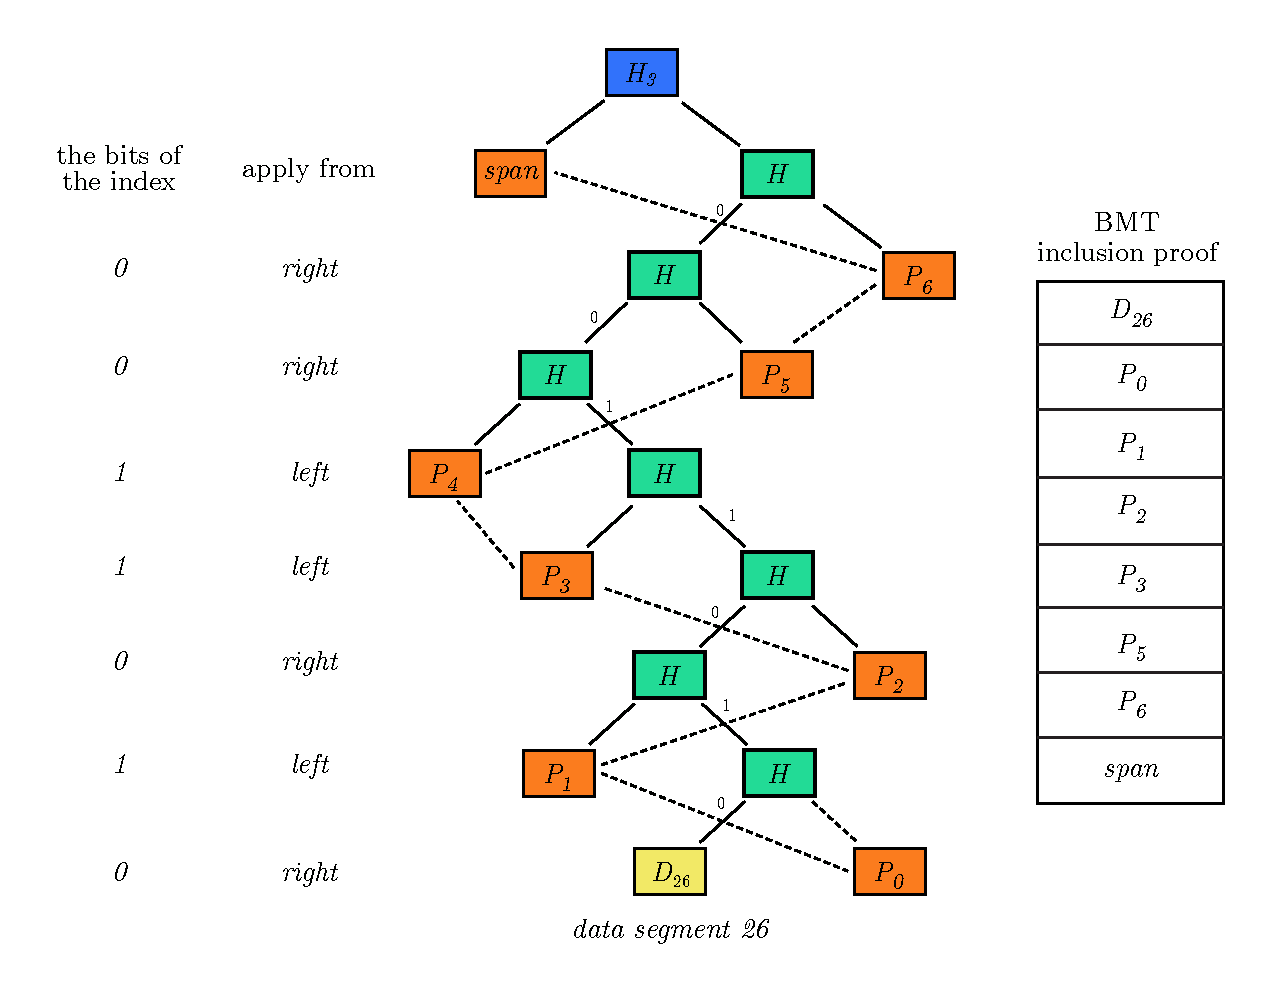
\includegraphics[width=\textwidth]{fig/inclusion-proof.pdf}
\caption[Compact segment inclusion proofs for chunks ]{Compact segment inclusion proofs for chunks. Assume we need proof for segment 26 of a chunk (yellow). The orange hashes of the BMT are the sister nodes on the path from the data segment up to the root and constitute what needs to be part of a proof. When these are provided together with the root hash and the segment index, the proof can be verified. The side on which proof item $i$ needs to be applied depends on the $i$-th bit (starting from least significant) of the binary representation of the index. Finally the span is prepended and the resulting hash should match the chunk root hash.}
\label{fig:chunk-inclusion}
\end{figure}

\begin{definition}[BMT segment inclusion proof \statusgreen]
\label{def:sip}
Define  $\mathit{SIP}(c,i)$ as the $\mathit{BMT}$ inclusion proof on chunk $c$ for segment index $i$.

\begin{eqnarray}
\mathit{SIP}&: &\mathit{Chunks}\times \overline{0,127} \mapsto \mathit{SIP}\\
\mathit{SIP} &:=&\mathit{Segment}\times\mathit{Segment}^7\times \mathit{byte}\{8\}
\\
\mathit{SIP}(c,i) &\defeq &\langle \mathit{Segment}(c,i),\langle h_0, h_1, \ldots, h_6\rangle, \mathit{span}(c)\rangle  
\end{eqnarray}
where
\begin{eqnarray}
h_j&\defeq& \mathit{BMT}(s_j,j)\\
s_j&\defeq&\mathit{Segment}(c,\mathit{start}(i,j))\concat \ldots \concat \mathit{Segment}(c,\mathit{start}(i,j)+2^j)\\
\end{eqnarray}
where
\begin{eqnarray}
\mathit{start}(i,j)&\defeq&
\begin{cases}
0 &\text{if } j=7\\
start(i,j+1)+2^{j-1}\cdot (\mathit{int}(i\cdot 2^{-j}) \mod 2) &\text{otherwise}
\end{cases}
% +\Sigma_{k=0}^j 2^j(\cdot (\mathit{int}(i\cdot 2^{-k}) \mod 2)-1) 
% _{\mathit{int}(i\cdot 2^{-(j+1)})\cdot s\cdot 2^{j+1} + 2^j\cdot(\mathit{int}(i\cdot 2^{-(j+1)})\mod 2)
% k = \mathit{exp}_2(j)
\end{eqnarray}
\end{definition}


\begin{definition}[BMT SIP validation \statusgreen]
\label{def:sip-validation}
Define  $\mathit{Valid}[\textsc{\lowercase{SIP}}](a, i, p)$ as the validator of a BMT segment inclusion proof $p$ for chunk at address $a$ on segment index $i$.

\begin{eqnarray}
\mathit{Valid}[\textsc{\lowercase{SIP}}]&:&\mathit{Segment}\times\overline{0,127}\times \mathit{SIP} \mapsto \{\mathtt{T,F}\}
\\
\mathit{Valid}[\textsc{\lowercase{SIP}}](a,i,p) &\Leftrightarrow&
\mathit{H}(m\concat a_7)=a
\end{eqnarray}where\begin{eqnarray}
a_0 &\defeq& d \\
a_{j+1}&\defeq& \begin{cases}
\mathit{H}(a_j\concat h_j) & \text{if }\mathit{int}(i\cdot2^{-j}) \mod 2 = 1\\
\mathit{H}(h_j\concat a_j) &\text{otherwise}
\end{cases}\text{ and }\\
p &= &\langle d,\langle h_0, h_1, \ldots, h_6\rangle, m\rangle
\end{eqnarray}
\end{definition}

 
\begin{definition}[Single owner chunks data integrity proof \statusgreen]
\label{def:socproof}
Define a single owner chunk storage proof $\Pi[\textsc{\lowercase{SOC}}](c,i)$ as a segment inclusion proof of the data payload of SOC $c$ on index $i$ together with the ID and signature of SOC $c$.

\begin{eqnarray}
\Pi[\textsc{\lowercase{SOC}}] &:&\mathit{SOC}\times\overline{0,127}\mapsto\mathit{SIP}\times\mathit{Sig}\times\mathit{Segment}\\ 
\Pi[\textsc{\lowercase{SOC}}](\langle o,id,data\rangle,i)&\defeq&  \langle e, sig, id\rangle
\end{eqnarray}where\begin{eqnarray}
e&=&\mathit{SIP}(data,i)\\
sig&=&\mathit{Sig}(o,id\concat \mathit{root}(e))
\end{eqnarray}
\end{definition}

\begin{definition}[Single owner chunks data integrity validation  \statusgreen]
\label{def:socproof-validity}
Define $\mathit{Valid}[\textsc{\lowercase{SOC}}](a, i, p)$ as the validator of a single owner chunk storage proof $p$ for chunk at address $a$ on segment index $i$.

\begin{eqnarray}
\mathit{Valid}&:&\mathit{Address}\times\overline{0,127}\times\Pi[\textsc{\lowercase{SOC}}]\mapsto\{T,F\}\\ \mathit{Valid}(a, i, \langle p, sig, id\rangle)&
\Leftrightarrow&\\
\text{payload } a'&=& \mathit{root}(p) \text{ such that } \mathit{Valid}(root(p),i,p)\\
\text{owner } o&=& \mathit{ECRecover}(sig,id\concat a')\\
\text{address } a&=& \mathit{H}(id\concat o)
\end{eqnarray}
\end{definition}

\begin{definition}[chunking \statusgreen]
\label{def:chunking}
The \emph{split} function splits an arbitrary byte slice into chunks.
\begin{eqnarray}
\mathit{split}&:&\mathit{byte}{*}\mapsto\mathit{Chunk}{*}\\
\mathit{split}(d)&\defeq&\langle c_0, c_1, \ldots c_{n-1}\rangle\\
\end{eqnarray}
such that
\begin{eqnarray}
c_i&=&\mathit{CAC}(d[o\rangedel o+l],l)\\
&&\text{for }0\leq i<\mathit{int}( \frac{\mathit{len}(d)-1}{4096})+1
\\
\text{offset }o&=&i\cdot 4096\\
\text{length }l&=&\begin{cases}
\mathit{len}(d)-o&\text{if }o+4096>\mathit{len}(d)\\
4096&\text{otherwise}
\end{cases}
\end{eqnarray}
\end{definition}

\begin{definition}[Swarm file level chunks $\Psi$ \statusgreen]
\label{def:lambda}
\begin{eqnarray}
\Psi&:&\mathit{byte}{*}\mapsto\mathit{uint8}\mapsto\mathit{Chunks}{*}\\
\text{data chunks }\Psi(d,0)[i] &\defeq&\mathit{split}(d)[i]\\ 
&&\text{for }0\leq i< \mathit{len}(\mathit{split}(d))\\
\text{intermediate chunks }\Psi(d,j)[i]&\defeq&\mathit{Pack}( 
\Psi(d,j-1)[o],\ldots,\Psi(d,j-1)[o+l])\\
&&\text{for }0\leq i<\mathit{len}(\Psi(d,j-1))\\
\text{offset }o&=&i\cdot 128\\
\text{length }l&=&\begin{cases}
\mathit{len}(\Psi(d,j-1))-o&\text{if }o+128>\mathit{len}(\Psi(d,j-1))\\
128&\text{otherwise}
\end{cases}
\end{eqnarray}
where
\begin{eqnarray}
\mathit{Pack}&:&\mathit{Chunks}^m\mapsto\mathit{Chunks}\\
\mathit{Pack}(c_0,\ldots ,c_{n-1})&\defeq&
\begin{cases}
c_0&\text{if }n=1\\
\mathit{CAC}(\Concat_{i=0}^{n-1}\mathit{Address}(c_i),\sum_{i=0}^{n-1}\mathit{span}(c_i))&\text{otherwise}
\end{cases}
\end{eqnarray}
Define the swarm file hash root chunk as $\mathit{Root}(d) = \Psi(d,j)[0]$ with the smallest $j$ such that $\mathit{len}(\Psi(d,j))=1$. We define $j$ as the \emph{Depth} of (the swarm representation of the file) data $d$.  
\end{definition}

\begin{definition}[Swarm File Hash $\mathit{H}^{+}$ \statusgreen]
\label{def:swarm-hash}
\begin{eqnarray}
\mathit{H}^{+}&:&\mathit{byte}{*}\mapsto\mathit{Address}\\
\mathit{H}^{+}(d)&\defeq&\mathit{Address}(\mathit{Root}_{\Psi}(d))
\end{eqnarray}
\end{definition}

\begin{definition}[Random access path for files \statusgreen]
\label{def:random-access-path}
Define the random access path $\tau(d,i)$ for file $d$ as the sequence of chunks in the the swarm hash tree leading from the root chunk via intermediate chunks to the data chunk containing segment $i$.

\begin{eqnarray}
\tau&:&\mathit{byte}{*}\times\mathit{uint64}\mapsto\mathit{Chunks}^m\\
\tau(d, j)&\defeq&\langle c_0, c_1, \ldots c_{n-1}\rangle
\end{eqnarray}
such that
\begin{eqnarray}
c_i&\defeq&
\begin{cases}
\mathit{Root}_\Psi(d)&\text{if }i=0\\
\mathit{Segment}(c_{i-1}, \mathit{index}(c_{i-1}, 32\cdot j))&\text{otherwise} 
\end{cases}
\end{eqnarray}
where
\begin{eqnarray}
\mathit{index}&:&\mathit{Chunks}\times\mathit{uint64}\mapsto\overline{0,127}\\
\mathit{index}(c, o)&\defeq&\mathit{int}\left(\frac{k}{m}\right)\\
\text{offset within subtree }k&=&o \mod 128^{\mathit{depth}(c)}\\
\text{max span of children } m&=&128^{\mathit{depth}(c)-1}
\end{eqnarray}
and
\begin{eqnarray}
\mathit{depth}&:&\mathit{Chunks}\mapsto \mathit{uint8}\\
\mathit{depth}(s)&\defeq&\Psi \text{ such that } 128^{\Psi-1}<\mathit{span}(c)\leq 128^\Psi
\end{eqnarray}
\end{definition}

\begin{definition}[Segment inclusion proof for files \statusgreen]
\label{def:sip+}
Define the Segment Inclusion Proof $\Pi[\textsc{\lowercase{SIP}}^{+}](d, j)$ for file $d$ as the series of chunk-inclusion proofs of the random access path to the segment at index  $j$.

\begin{eqnarray}
\Pi[\textsc{\lowercase{SIP}}^{+}]&:&\mathit{byte}{*}\times\mathit{uint64}\\
\Pi[\textsc{\lowercase{SIP}}^{+}](d, j)&\defeq&\langle p_0, p_1, \ldots p_{n-1}\rangle
\end{eqnarray}
such that
\begin{eqnarray}
p_i&\defeq&
\Pi[\textsc{\lowercase{SIP}}](\tau(d,j)[i], \mathit{index}(\tau(d,j)[i],32\cdot j))
\end{eqnarray}
\end{definition}

\begin{definition}[Segment Inclusion Proof validity for files \statusgreen]
\label{def:sip+-validity}
Define the validator function $\mathit{Valid}[\textsc{\lowercase{SIP}}^{+}](a,s,j,p)$ for Segment Inclusion Proof $p$ for a file with swarm hash $a$ having segment $s$ at index  $j$.

\begin{eqnarray}
\mathit{Valid}[\textsc{\lowercase{SIP}}^{+}]&:&\mathit{Address}\times\mathit{Segment}\times\mathit{uint64}\times\Pi[\textsc{\lowercase{SIP}}^{+}]\mapsto\{\mathtt{T,F}\}\\
\mathit{Valid}[\textsc{\lowercase{SIP}}^{+}](a,s,j,p)&\Leftrightarrow&\\
&&\mathit{Valid}[\textsc{\lowercase{SIP}}](a_{i+1}, a_i,j,p_i)
\text{ for }0\leq i<n\\
&&a_n=a
\end{eqnarray}
where
\begin{eqnarray}
p&=&\langle p_0, p_1, \ldots, p_{n-1}\rangle\\
a_0&=&s
\end{eqnarray}
\end{definition}



\subsubsection{Reserve size}
\begin{definition}[Segment transform \statusgreen]
\label{def:st}
Define  $\mathit{ST}(s,n,k)$ as the node-specific  transform of a 
segment $s$ with nonce $k$ for node $n$.

\begin{eqnarray}
\mathit{ST}&: &\mathit{Segment}\times\mathit{Nodes}\times  \mathit{Nonce}\mapsto \mathit{Segment}
\\
\mathit{ST}(s,n,k) &\defeq &
s\xor \mathit{Overlay}(n) \xor k
\end{eqnarray}
\end{definition}



\begin{definition}[Single segment transform \statusgreen]
\label{def:sst}
Define  $\mathit{SST}(c,n,k)$ as the single segment transform of a chunk $c$ with nonce $k$ for node $n$.

\begin{eqnarray}
\mathit{SST}&: &\mathit{Chunk}\times\mathit{Nodes}\times  \mathit{Nonce}\mapsto \mathit{Chunk}
\\
\mathit{CST}(c,n,k) &\defeq &c'\\
\mathit{Segment}(c',i)&\defeq&\begin{cases}
\mathit{ST}(\mathit{Segment}(c,i), n, k)& \text{if } i = k  \mod sc\\
\mathit{Segment}(c,i) & \text{otherwise for all } 0<=i<sc 
\end{cases}
\end{eqnarray}
where
\begin{eqnarray}
\text{segment count} &sc =&\frac{\mathit{len}(c)-1}{32}+1 
\end{eqnarray}
\end{definition}

\begin{definition}[Single segment transform proof \statusgreen]
\label{def:sst-proof}
Define the single segment transform proof for chunk $c$ for node $n$ with nonce $k$ as the BMT SIP of the chunk on segment index $i$ where $i$ is $k$ modulo the number of segments covering the data for chunk $c$.


\begin{eqnarray}
\Pi[\textsc{\lowercase{SST}}] &:& \mathit{Chunks}\times\mathit{Nonce}\mapsto\mathit{SIP}\\
\Pi[\textsc{\lowercase{SST}}](c,k) &\defeq& \mathit{SIP}(c,i) 
\end{eqnarray}
where
\begin{eqnarray}
\text{\sc{sip} index } i&=&k \mod \frac{\mathit{len}(c)-1}{32}+1
\end{eqnarray}
\end{definition}


\begin{definition}[Single segment transform validation \statusgreen]
\label{def:sst-validation}
Define $\mathit{Valid}[\textsc{\lowercase{SST}}](a, a', n, k, p)$ as the validator function for single segment proof $p$ for node $n$ with nonce $k$ on original chunk address $a$, and SST address $a'$.

\begin{eqnarray}
\mathit{Valid}[\textsc{\lowercase{SST}}]&:& 
%\mathit{Segment}\times\mathit{SIP}\times\mathit{Stamps}\times
\mathit{Address}^2\times\mathit{Nodes}\times\mathit{Nonce}\times\mathit{SIP}\mapsto \{\mathtt{T,F}\}
\\
\mathit{Valid}[\textsc{\lowercase{SST}}](a,a',n,k,p)&\Leftrightarrow&\\
\text{original}&&\mathit{Valid}[\textsc{\lowercase{SIP}}](a, i, p)\land\\
\text{transformed}&&\mathit{Valid}[\textsc{\lowercase{SIP}}](a', i, p')
\end{eqnarray}
given
\begin{eqnarray}
\text{segment index } i &=&k \mod\frac{\mathit{len}(m)-1}{32}+1\\
 \text{original proof } p& = &\Pi[\textsc{\lowercase{SST}}](c,k)=    \langle d,h, m\rangle\\
 \text{\sc{sst} proof } p' &=&\langle \mathit{ST}(d,n,k),h, m\rangle
\end{eqnarray}
\end{definition}


\begin{definition}[Reserve commitment \statusgreen]
\label{def:RC}
Define $\mathit{RC}(C,n,k)$ as the reserve commitment by node $n$ with nonce $k$ over the sample sequence $C$ of chunks.
\begin{eqnarray}
\mathit{RC}&:&(\mathit{Chunks}^{m})\times\mathit{Nodes}\times\mathit{Nonce}\mapsto\mathit{byte}{*}\\
\mathit{RC}(C,n,k)&\defeq&\Concat_{i=0}^{m}(d_i\concat sth_i)
\end{eqnarray}
where
\begin{eqnarray}
\text{{\sc rc} even segments } 
d_i&\defeq&\mathit{BMT}(\mathit{SST}(\mathit{data}(c_i),n,k), \mathit{meta}(c_i))\\
\text{{\sc rc} odd segments } sth_i&\defeq& \mathit{H}(\mathit{Stamp}(c_i))\\
\text{sample sequence } C&=&\langle c_0, c_1, \ldots, c_{m-1}\rangle
\end{eqnarray}
\end{definition}

\begin{definition}[Reserve commitment hash \statusgreen]
\label{def:RCH}
Define $\mathit{RCH}(C,n,k)$ as the swarm file hash of reserve commitment by node $n$ with nonce $k$ over the sample sequence $C$ of chunks.
\begin{eqnarray}
\mathit{RCH}&:&(\mathit{Chunks}^{m})\times\mathit{Nodes}\times\mathit{Nonce}\mapsto\mathit{Address}\\
\mathit{RCH}(C,n,k)&\defeq&\mathit{H}^{+}(\mathit{RC}(C,n,k))
\end{eqnarray}
\end{definition}


\begin{definition}[Proof of reserve \statusgreen]
\label{def:RC-proof}
Define $\Pi[\textsc{\lowercase{RC}}](C,n,k,k')$, proof of reserve for chunkset $C$, node $n$ and nonces $k$ and $k'$ as the extended segment inclusion proof on the reserve commitment $rc=\mathit{RC}(C,n,k)$.
\begin{eqnarray}
\Pi[\textsc{\lowercase{RC}}]&:&(\mathit{Chunks}^{m})\times\mathit{Nodes}\times\mathit{Nonce}^2\mapsto\mathit{SIP}^{+}\times\mathit{Stamp}\\
\Pi[\textsc{\lowercase{RC}}](C,n,k,k')&\defeq&\langle\mathit{SIP}^{+}(\mathit{RC}(C,n,k),2\cdot i), \mathit{Stamp}(c_i)\rangle
\end{eqnarray}
where
\begin{eqnarray}
\textsc{sip}^{+}\text{ index } i&=&k' \mod m\ (=\lvert C\rvert)\\
\text{sample sequence } C&=&\langle c_0, c_1, \ldots, c_{m-1}\rangle
\end{eqnarray}
\end{definition}

\begin{definition}[Proof of reserve validation \statusgreen]
\label{def:RC-proof-validity}
Define $\mathit{Valid}[\textsc{\lowercase{RC}}](a, i, p)$ as the validation function for reserve commitment $p$ having address $a$ at index $i$.

\begin{eqnarray}
\mathit{Valid}[\textsc{\lowercase{RC}}]&:&\mathit{Address}\times\mathit{Nonce}\times(\mathit{SIP}^{+}\times\mathit{Stamp})\mapsto\{\mathtt{T,F}\}\\
\mathit{Valid}[\textsc{\lowercase{RC}}](a,k,p)&\Leftrightarrow&\\
\text{inclusion } && \mathit{Valid}[\textsc{\lowercase{SIP}}^{+}](a,i,p)\\
\textsc{SIP}^{+}\text{ index } && i=k \mod \frac{\mathit{span}(p)}{64}
\end{eqnarray}
\end{definition}


\begin{definition}[Proof of retention in reserve validation \statusgreen]
\label{def:RC-retention-proof-validity}
Define $\mathit{Valid}[\textsc{\lowercase{RC-SST}}](a, n, k, k', p, p')$ as the validation function for a combination of reserve commitment proof $p$ and single segment transform proof $p'$ for node $n$ and nonce $k$ having swarm address $a$ at index derived from $k'$.

\begin{eqnarray}
\mathit{Valid}[\textsc{\lowercase{RC-SST}}]&:&\mathit{Address}\times\mathit{Nodes}\times\mathit{Nonce}^2\\
&&\times(\mathit{SIP}^{+}\times\mathit{Stamp})\times\mathit{SIP}\mapsto\{\mathtt{T,F}\}\\
\mathit{Valid}[\textsc{\lowercase{RC-SST}}](a, n, k, k', p, p')&\Leftrightarrow&\\
\text{{\sc RC} inclusion } && \mathit{Valid}[\textsc{\lowercase{RC}}](a',k',p)\\
\text{chunk retention } && \mathit{Valid}[\textsc{\lowercase{SST}}](a,a',n,k,p')
\end{eqnarray}
\end{definition}


\subsubsection{Participation}

\begin{definition}[Push-sync request \statusgreen]
\label{def:push-sync-request}
Define  $\mathit{Request}(c,st)$ as the request  to instruct swarm to store chunk $c$ with postage stamp $st$ originating from requester $o=\mathrm{owner}(st)$. 

\begin{eqnarray}
\mathit{Requests}&\defeq&\mathit{Chunks}\times\mathit{Stamps}\\ 
\langle c, st\rangle\in\mathit{Requests} \\
&\Leftrightarrow&\\
\text{chunk}&c&\text{chunk to be uploaded}\\
\text{stamp}&st&\text{valid postage stamp}\\
\text{originator } o&=&\mathrm{owner}(st)
\end{eqnarray}
% where\begin{eqnarray}
% c&\defeq&
% \end{eqnarray}
\end{definition}

\begin{definition}[Receipt \statusgreen]
\label{def:receipt}
Define  $\mathit{Receipt}(n,st)$ as the receipt issued by node $n$ on chunk request with stamp $st$.

\begin{eqnarray}
\mathit{Receipt}&:&\mathit{Nodes}\times\mathit{Stamps}\times\mapsto\mathit{Receipts}\\ 
\mathit{Receipts} &\defeq&
\mathit{Address}\times\mathit{Segment}\times\mathit{Nodes}\times\mathit{Timestamp}\\
\mathit{Receipt}(n, st) &\defeq& \langle
a, g, m, t \rangle
\end{eqnarray}
where
\begin{eqnarray}
\text{address } a&=&\mathit{Address}(st)\\
\text{commit } g&=&\mathit{RCH}(n,k) \text{ for some }k\\
\text{closest node } m&=&\operatorname{arg\,max}_{j\in\mathit{Neighbours}(n)}\mathit{PO}(a,j)\\
\text{timestamp } t&=&\texttt{NOW} \text{-- time of issuing receipt}
\end{eqnarray}
and authenticated version (signed receipts):
\begin{eqnarray}
\mathit{Receipts}_S &\defeq&\mathit{Sig}\times\mathit{Receipts}
 \end{eqnarray}

\end{definition}

\begin{definition}[Receipt validity \statusgreen]
\label{def:receipt-validity}
Define  $\mathit{Valid}[\textsc{\lowercase{REC}}](st,\langle sig,r\rangle)$ as the validator function for a signed receipt $\langle sig,r\rangle$ as response to a pushed chunk request with stamp $st$. Receipt validity check is performed by the request originator.

\begin{eqnarray}
\mathit{Valid}[\textsc{\lowercase{REC}}] &:&\mathit{Stamp}\times\mathit{Receipts}_S\mapsto\{\mathtt{T,F}\}\\
\mathit{Valid}[\textsc{\lowercase{REC}}](st,\langle sig,\langle
a, g, m, t \rangle\rangle)\\
&\Leftrightarrow&\\
\text{valid timestamp } &&\mathit{Time}(r)<t<\mathtt{NOW}\\
\text{storer in neighbourhood} && \mathit{PO}(a,n)\geq \mathit{depth}\\
\text{closest node is closer} && \mathit{PO}(a,m)\geq\mathit{PO}(a,n)
\end{eqnarray}
where
\begin{eqnarray}
a&=&\mathit{Address}(st)\\
n&= &\mathit{ECRecover}(sig,r)
\end{eqnarray}
\end{definition}


\begin{definition}[Proof of participation \statusgreen]
\label{def:pop}
Define  proof of participation $p=\Pi[\textsc{\lowercase{PART}}](n, st)$ for node $n$
and chunk request $q=\langle c,st\rangle$ as the receipt issued by storer $n$ on request $q$ countersigned by the batch owner of stamp $st$.

\begin{eqnarray}
\Pi[\textsc{\lowercase{PART}}] &:& \mathit{Nodes}\times\mathit{Stamps}\mapsto \mathit{Receipts}_S\\
\Pi[\textsc{\lowercase{PART}}](n,st) &\defeq&  \langle\mathit{Sig}(\mathrm{owner}(st),n\concat r), r\rangle
\end{eqnarray}
where
\begin{eqnarray}
r &=& \mathit{Receipt}(n, st)
\end{eqnarray}
\end{definition}


\begin{definition}[Proof of participation validity \statusgreen]
\label{def:pop-validity}
Define $\mathit{Valid}[\textsc{\lowercase{PART}}](n,st,p)$ as the validator of a proof of participation $p$ for node $n$ with chunk at address $a$ and stamp $st$.
\begin{eqnarray}
\mathit{Valid}[\textsc{\lowercase{PART}}]  &:& \mathit{Nodes}\times\mathit{Stamp}\times\mathit{Part}\mapsto \{\mathtt{T,F}\}\\
\mathit{Valid}[\textsc{\lowercase{PART}}](n,st,\langle sig, r\rangle)\\
&\Leftrightarrow&\\
\text{countersigned by owner} && \mathrm{owner}(st) = \mathit{ECRecover}(sig, n\concat r) \\
\text{relevant chunk}&&\mathit{Valid}[\textsc{\lowercase{STAMP}}](st)\\   
\text{receipt valid}&&\mathit{Valid}[\textsc{\lowercase{REC}}](st,r)
\end{eqnarray}
\end{definition}

\subsection{The lottery}

\begin{definition}[Lottery \statusred]
\label{def:lottery} 
\begin{eqnarray}
\end{eqnarray}
\end{definition}

\begin{definition}[Ticket \statusred]
\label{def:ticket}
A ticket is defined as a tuple comprising all types of evidence:
(1) participation ($\Pi[\textsc{\lowercase{PART}}]$), (2) reserve uniformity ($\Pi[\textsc{\lowercase{RC}}]$), (3) retention ($\Pi[\textsc{\lowercase{DATA}}]$) (4) relevance ($\Pi[\textsc{\lowercase{REL}}]$) 
\begin{eqnarray}
\mathit{Tickets}&\defeq&\mathit{Header}\times\textsc{PAR}\times\textsc{RES}\times\textsc{REL}\times\textsc{DATA}
\end{eqnarray}
\end{definition}


\begin{definition}[Ticket validity \statusred]
\label{def:ticket-validity}

\end{definition}

\begin{definition}[Winner claim \statusred]
\label{def:winner-claim}

\end{definition}

\begin{definition}[Winner claim validity \statusred]
\label{def:winner-claim-validity}

\end{definition}


\begin{definition}[Recent tickets \statusred]
\label{def:recent-tickets}
\begin{eqnarray}
\mathit{}&:&\\
\mathit{}&\defeq&
\end{eqnarray}
\end{definition}

\begin{definition}[Neighbourhood active nodes set \statusred]
\label{def:nans}
Define neighbourhood active nodes set $\mathit{NANS}(N,\lambda,k)$
for neighbourhood $N$ and lottery index $\lambda$ as the set of nodes selected by the input nonce $k$.
\begin{eqnarray}
\mathit{NANS}&:&\mathit{Neighbourhood}\times\mathit{uint64}\times\mathit{Segment}\mapsto\mathcal{P}(\mathit{Nodes})\\
\mathit{NANS}(N,\lambda,k)&\defeq&
\end{eqnarray}
where
\begin{eqnarray}
i&=&k \mod \mathit{SegmentCount}(\mathit{span}(\mathit{RC}))
\end{eqnarray}
\end{definition}

\subsection{Lottery draw}  

\begin{definition}[Storage lottery on the blockchain\statusred]
\label{def:lottery-blockchain}
Define lottery $\Lambda$ as an evaluation context the state of which is under the consensus of the blockchain, tracked by discreet time indexes (block height).

\begin{eqnarray}
\textsc{State}&:&\mathit{uint64}\mapsto\mathit{Address}^4\times\mathit{uint64}\\
\textsc{State}(\lambda)&\defeq&
\end{eqnarray}

\end{definition}


\newpage
\begin{definition}[Honest node screenplay\statusorange]
\label{def:honest-node-screenplay}
Define the \emph{honest node screenplay} as the intended  strategy honest nodes should be following.

\begin{itemize}[noitemsep]
\item[\textsc{\lowercase{block}}]
\item[]\begin{itemize}[noitemsep]
\item[(0)] watch blockchain contract logs and subscribe to a lottery draw event
\item[(1)]     
set current chain head to new lottery nonce as per the event log
\item[(2)] (re)start    (\textsc{peers}) 
\item[(3)] (re)start    (\textsc{chunk}) 
\item[(4)] repeat (\textsc{block})
\end{itemize}

\item[\textsc{\lowercase{peers}}]
\item[]\begin{itemize}[noitemsep]
\item[(0)]    
listen to nearest neighbours broadcast of their chains, 
\item[(1)]    
compare this chain with our own, repeat (\textsc{peers}) unless better
\item[(2)] 
verify chain and  repeat (\textsc{peers}) unless valid 
\item[(3)]    
reset current chain, 
\item[(4)]    
abort and restart (\textsc{commit})
\item[(5)]    
abort and restart (\textsc{chunk})
\item[(4)] repeat (\textsc{peers})
\end{itemize}

\item[\textsc{\lowercase{chunks}}]
\item[]\begin{itemize}[noitemsep]
\item[(0)]    
receive push-synced chunk  
\item[(1)] include reserve commitment
\item[(2)] 
\item[(3)] attach and sign, respond with receipt
\end{itemize}

\item[\textsc{\lowercase{tickets}}]
\item[]\begin{itemize}[noitemsep]
\item[(4)] receive the attestation, or timeout and repeat (\textsc{chunk})
\item[(5)] check if winning or repeat (\textsc{tickets}) 
\item[(6)] wrap ticket and append to chain as new head
\item[(7)] broadcast new chain to neighbours
\item[(8)] if chain length less than \texttt{TOKEN\_COUNT}, repeat (\textsc{chunk})
\item[(9)] continue (\textsc{chunk})
\end{itemize}
\item[\textsc{\lowercase{commit}}]
\item[]\begin{itemize}[noitemsep]
\item[(0)] finalise currently built segment transform of the reserve
\item[(1)]assign root hash to history
\item[(2)] finalise current state of the reserve 
\item[(3)] start iteration on it to recalculate single segment transform
\end{itemize}
\item[\textsc{\lowercase{win}}]
\item[]\begin{itemize}[noitemsep]
\item[(0)] provide/collect all inclusion proofs for all the tickets
\item[(1)] wrap claim in transaction and sign
\item[(2)] broadcast tx to neighbourhood and submit to blockchain
\end{itemize}
\end{itemize}
\end{definition}

\begin{definition}[Claim validation screenplay\statusorange]
\label{def:lottery-claim-validation}
Define claim validation screenplay as the formulation of postage lottery contract submit claim call. At each step if condition not met, reject and rollback.
\begin{itemize}[noitemsep]
\item[(0)]    
verify initial nonce matches open lottery nonce
\item[(1)]
calculate expected length of chain from interval and blockheight of last payout
\item[(2)]    
verify length of chain equals expected length
\item[(3)]
verify at least r nodes submitted ticket
\item[(4)]    
verify timestamps of postage stamps of tickets are in order
\item[(5)] 
verify for each ticket's familiarity
\item[(6)]
for each ticket, node and chunk is within reserve radius of the lottery anchor
\item[(7)] 
calculate total to be send out
\item[(8)]
for each ticket, verify validity of proof of reserve selects identical underlying  chunk
\item[(9)]
calculate average density both historically and over proofs of reserve size
\item[(10)]
record current density, recalculate unit price
\item[(11)]
adjust outpayment and transfer amounts
\item[(12)]
remove expired batches
\item[(13)]
recalculate prompt interval
\item[(14)]
set new nonce input and emit draw event
\end{itemize}
\end{definition}

\begin{definition}[Lottery draw calibration\statusred]
\label{def:lottery-draw-calibration}

\end{definition}

\begin{definition}[Winner's claim\statusred]
\label{def:claim}

\end{definition}

\begin{definition}[Winner's claim validation\statusred]
\label{def:claim-validation}

\end{definition}